\documentclass[11pt,a4paper]{report}

\usepackage[utf8]{inputenc}
\usepackage{amsmath}
\usepackage{amsfonts}
\usepackage{amssymb}
\usepackage{graphicx}
\usepackage[left=2cm,right=2cm,top=2cm,bottom=2cm]{geometry}
\usepackage{amsmath}
\usepackage{wrapfig}

\title{ARPA: Autonomous Robotic Pointer Arm}
\author{Helgerud, Erlend \and Håland, André}

\begin{document}
	\maketitle
	\tableofcontents
	\newpage

	%\section{Abstract}
	%\section{Introduction}
	%\section{Related works}
	\section{System description}
	
	\subsection{Architecture}
	ARPA is divided into nodes. These nodes each has its own tasks and communicate with each other on different topics to exchange information. Figure \ref{fig:nodegraph} shows the nodes of ARPA, and the topics they communicate on. A circle represents a node, whilst a rectangle represents a topic. The controller node is the center of all actions. It handles the interface between the camera, MATLAB, the physical robotic arm and the model in gazebo. The camera node is currently just a mock-up which sends a Cartesian point in space to the controller. The MATLAB node handles inverse kinematics. It receives Cartesian coordinates from the controller, and sends back five joint angles. The 5DOF Robot node controls the physical robotic arm by writing received angles to the servo motors. The Gazebo node listens to the same topics as 5DOF Robot, and will simulate a robotic model with a 1:1 relationship with the physical arm.
	
	\begin{figure}[ht]
		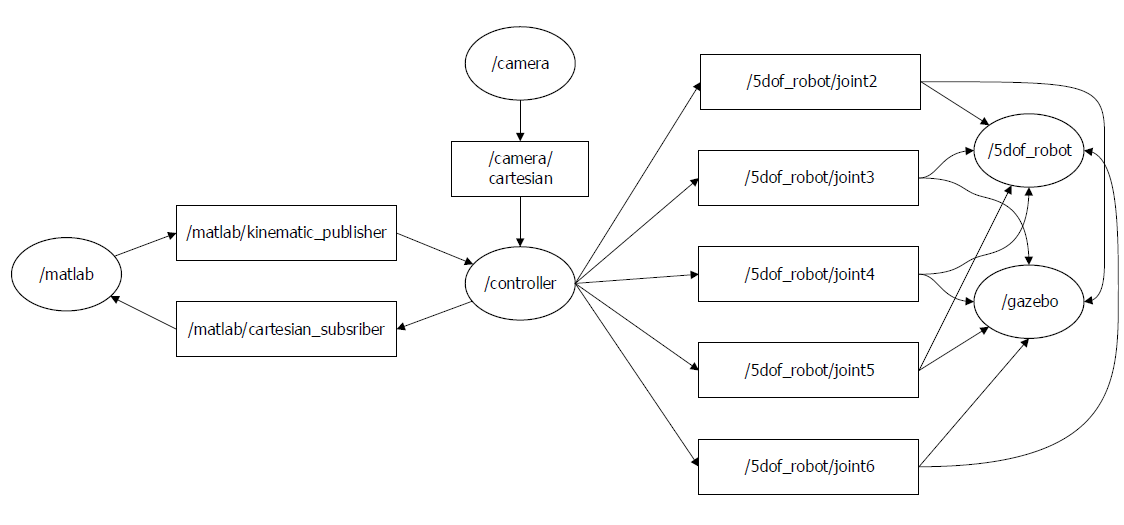
\includegraphics[width=\linewidth]{../Diagrams/NodeGraph.png}
		\caption{Node graph}
		\label{fig:nodegraph}
	\end{figure}
	
	\subsection{Information flow}
	
	The flow of information in ARPA starts with the camera getting a Cartesian coordinate of a dot in the workspace of ARPA. This coordinate is sent to the controller which further sends it to MATLAB for processing. MATLAB returns five joints angles to the controller. These are the angles used to control both the physical arm and the Gazebo model. Hence, the controller publishes them to their respective topics, where they are picked up by both the Gazebo node and the 5DOF Robot node. After the control node has sent the joint angles, it waits for 5 seconds before it sends a new set of joint angles used to set the physical and simulated arm back to starting position. Figure \ref{fig:seq-diagram} shows the flow of information in the form of a UML Sequence diagram.
	
	
	\begin{figure}[ht]
		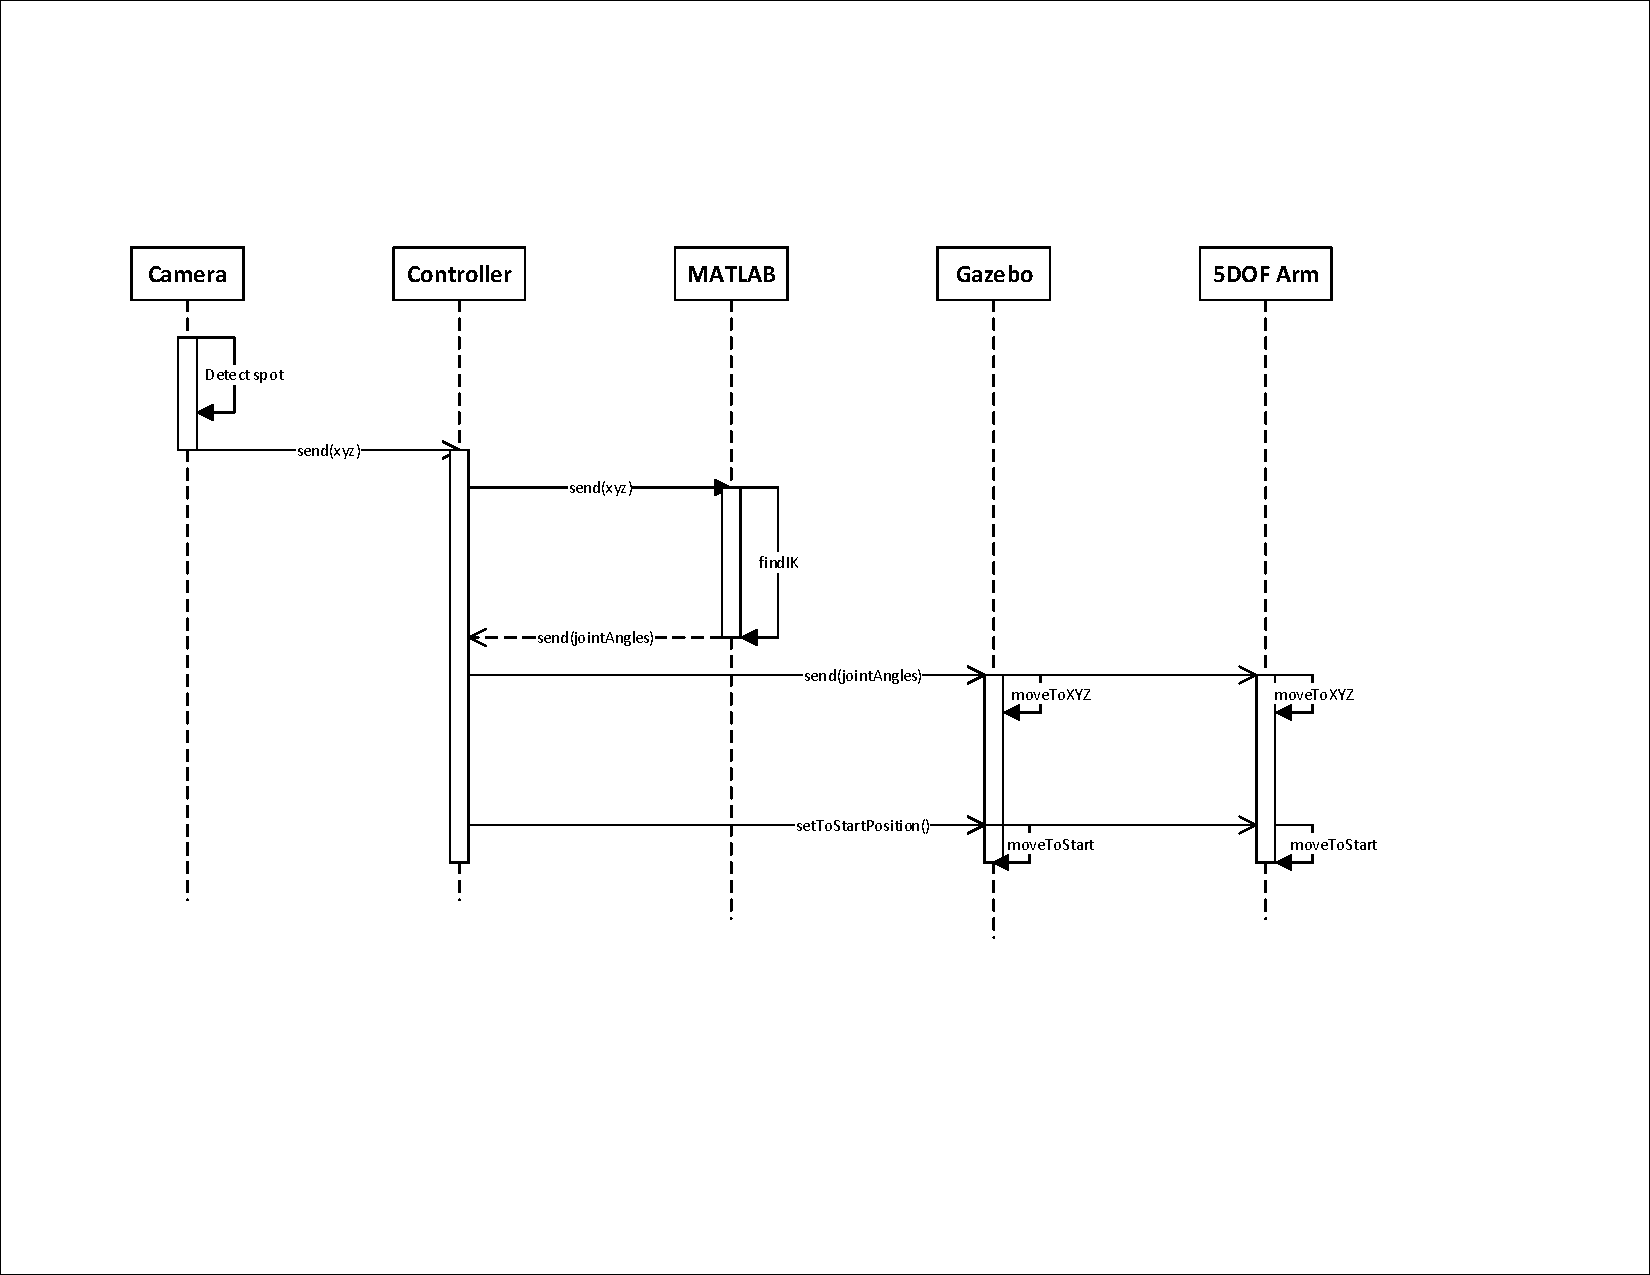
\includegraphics[width=\linewidth]{../Diagrams/SequenceDiagram.png}
		\caption{UML Sequence diagram}
		\label{fig:seq-diagram}
	\end{figure}
	
	%\section{Simulation and experiments}
	
	%\section{Discussion}
	
	%\section{Appendix}
	
	
\end{document}